\documentclass[class=scrartcl]{standalone}
\usepackage{chez}

\begin{document}
\section{Progress and preservation}
We will formalize what we mean when we say
``well typed programs never go wrong''.
In particular, we will prove this by induction:
\begin{itemize}
  \item If a program is well typed,
        it will stay well typed in the next step of evaluation.
  \item If a program is well typed, then either we are done
        or we can do another step of evaluations.
\end{itemize}
In order to do this, we need to formalize
what we mean by ``step of evaluation''.

% reference: the revised report of the syntactic theories
%            of sequential control and state
In contextual semantics, we have contexts that represent a `hole'
in which the next evaluation step will occur.
\[
  H \coloneq \bullet
        \mid H\, e_1
        \mid v\, H
        \mid H + e
        \mid v + H
        \mid \pifthenelse{H}{e_1}{e_2},
\]
where \(e\) is any expression and \(v\) is a fully evaluated expression.
We also have local reduction rules
\begin{itemize}
  \item \(n_1 + n_2 \to \pname{plus} n_1\, n_2\)
  \item \(\pifthenelse{\ptrue}{e_1}{e_2} \to e_1\)
  \item \(\pifthenelse{\pfalse}{e_1}{e_2} \to e_2\)
  \item \((\plambda{x \of \tau}{e_1}) v_2 \to e_1 [v_2/x]\)
\end{itemize}
and the global reduction rule
\[
  H[r] \to H[e] \iff r \to e.
\]

\begin{example}
  If we have \(((3 + 1) + 7) + (2 + 1)\),
  we have the following context:
  \begin{center}
    \begin{tikzpicture}
      \Tree [.\(+\) [.\(+\) [.\(\bullet\) ]
                    [.\(7\) ]]
                [.\((2+1)\) ] ]
    \end{tikzpicture}
  \end{center}

  Here are some more examples:
  \begin{center}
    \begin{tabular}{c c c}
      \toprule
      Expression & Context & Redex \\ \midrule
      \((\plambda{x \of \pint}{x + 1})(1+1)\) &
        \((\plambda{x \of \pint}{x + 1}) \bullet\) &
        \(1 + 1\) \\
      \((\plambda{x \of \pint}{x + 1})2\) &
        \(\bullet\) &
        \((\plambda{x \of \pint}{x + 1})2\) \\
      \(2 + 1\) &
        \(\bullet\) &
        \(2 + 1\) \\
      \bottomrule
    \end{tabular}
  \end{center}
\end{example}
For any expression, we can decompose it into a context and a redex.
Then, apply the reduction rule to the redex and repeat.

\subsection{Preservation}
When we used big-step semantics, we can prove global preservation.
In particular, we can prove this by induction on the structure of derivation
of \(e_1 \to e_2\).

\begin{adhoctheorem}{Recall}
  To prove \(Q(e) \implies P(e)\) by induction on the structure of derivation,
  \begin{enumerate}[nosep]
    \item Prove the base cases, i.e.\ prove \(P(e)\) holds for any \(e\)
          in which the proof tree for \(Q(e)\) has depth \(1\).
    \item Prove the inductive step, i.e.\ prove \(P(e)\) holds for any \(e\)
          in which the proof tree for \(Q(e)\) has height \(h+1\),
          assuming that \(P(e')\) holds for any \(e'\)
          in which the proof tree of \(Q(e')\) has height \(h\).
  \end{enumerate}
\end{adhoctheorem}

\begin{proposition}[Global preservation]
  \(e_1 \to e_2 \implies \Gamma \vdash e_1 \of \tau
                \implies \Gamma \vdash e_2 \of \tau\).
\end{proposition}
\begin{proof}
  We proceed by induction on \(e_2\).
  Here \(Q(e_1, e_2) = (e_1 \to e_2)\) and
  \(P(e_1, e_2) = (\Gamma \vdash e_1 \of \tau
                   \implies \Gamma \vdash e_2 \of \tau)\).

  \paragraph{Base cases}
  There are two base cases corresponding to
  \[
    \prfaxiom{x \to x} \qquad
    \prfaxiom{\lambda x. e \to \lambda x. e}
  \]
  In particular,
  \begin{gather*}
    \Gamma \vdash x \of \tau \implies \Gamma \vdash x \of \tau \\
    \Gamma \vdash \lambda x.e \of \tau
      \implies \Gamma \vdash \lambda x.e \of \tau
  \end{gather*}
  are both true.

  \paragraph{Inductive case}
  We have the operational rule
  \[
    \prftree{e_1 \to \lambda x. e_1'}
            {e_1'[e_2 / x] \to e_3}
            {e_1 e_2 \to e_3}
  \]
  We want to prove
  \[
    \Gamma \vdash e_1 e_2 \of \tau \implies \Gamma \vdash e_3 \of \tau,
  \]
  given the induction hypotheses
  \begin{gather}
    \forall t. (\Gamma \vdash e_1 \of t
      \implies \Gamma \vdash \lambda x. e_1' \of t) \label{preservation-1} \\
    \forall t. (\Gamma \vdash e_1'[e_2/x] \of t
      \implies \Gamma \vdash e_3 \of t). \label{preservation-2}
  \end{gather}
  
  From the typing rule
  \[
    \prftree{\Gamma \vdash e_1 \of \tau' \to \tau}
            {\Gamma \vdash e_2 \of \tau'}
            {\Gamma \vdash e_1 e_2 \of \tau}
  \]
  so we know there exists some \(\tau'\)
  such that \(\Gamma \vdash e_1 \of \tau' \to \tau\) and
  \(\Gamma \vdash e_2 \of \tau'\).
  By \cref{preservation-1},
  we have \(\Gamma \vdash \lambda x.e_1' \of \tau' \to \tau\).
  From the typing rule
  \[
    \prftree{\Gamma, x \of \tau' \vdash e_1' \of \tau}
            {\Gamma \vdash (\lambda x \of \tau' .\, e_1') \of \tau' \to \tau}
  \]
  we know that \(\Gamma, x \of t' \vdash e_1' \of \tau\).

  We use the following lemma:
  \begin{lemma}
    \[
      \Gamma, x \of \tau' \vdash e_1' \of \tau
        \land \Gamma \vdash e_2 \of \tau'
        \implies \Gamma \vdash e_1'[e_2 / x] \of \tau.
    \]
  \end{lemma}
  The proof is omitted as an exercise.
  The lemma yields \(\Gamma \vdash e_1'[e_2 / x] \of \tau\),
  and from \cref{preservation-2}, we have \(\Gamma \vdash e_3 \of \tau\).
\end{proof}


\subsection{Progress}
\begin{proposition}[Progress]
  If \(\vdash e \of \tau\) and \(e\) is not a value,
  then there exists \(e'\) such that \(e \to e'\)
  (equivalently, there exists \(H\) and \(r\) such that \(e = H[r]\)).

\end{proposition}
To prove progress, we want to use small step semantics,
because we want to talk about steps of evaluation.

\begin{proof}
  We prove this by induction on the derivation of \(\vdash e \of \tau\).
  
  \paragraph{Base cases:}
  We have the base cases
  \[
    \prfaxiom{\Gamma \vdash \ptrue \of \pbool} \qquad
    \prfaxiom{\Gamma \vdash \pfalse \of \pbool} \qquad
    \prfaxiom{\Gamma \vdash N \of \pint} \qquad
    \prftree{x \of \tau \in \Gamma}
            {\Gamma \vdash x \of \tau} \qquad
    \prftree{\Gamma, x \of \tau_1 \vdash e \of \tau_2}
            {\Gamma \vdash (\lambda x\of \tau_2 . e) \of \tau_1 \to \tau_2}
  \]
  Since these are irreducible values, the condition does not hold,
  so these vacuously satisfy the proposition.

  \paragraph{Inductive cases:}
  We have the inductive cases
  \[
    \prftree{\Gamma \vdash e_1 \of \tau' \to \tau}
            {\Gamma \vdash e_2 \of \tau'}
            {\Gamma \vdash e_1 e_2 \of \tau} \quad
    \prftree{\Gamma \vdash e_1 \of \pint}
            {\Gamma \vdash e_2 \of \pint}
            {\Gamma \vdash e_1 + e_2 \of \pint} \quad
    \prftree{\Gamma \vdash e_1 \of \pint}
            {\Gamma \vdash e_2 \of \pint}
            {\Gamma \vdash e_1 = e_2 \of \pbool} \quad
    \prftree{\Gamma \vdash e \of \pbool}
            {\Gamma \vdash e_t \of \tau}
            {\Gamma \vdash e_f \of \tau}
            {\Gamma \vdash \pifthenelse{e}{e_t}{e_f} \of \tau}
  \]
  We will do the proof for
  \[
    \prftree{\Gamma \vdash e \of \pbool}
            {\Gamma \vdash e_t \of \tau}
            {\Gamma \vdash e_f \of \tau}
            {\Gamma \vdash \pifthenelse{e}{e_t}{e_f} \of \tau}
  \]
  The rest of the cases are similar.
  By the inductive hypothesis,
  \(e\) is either a value or can be decomposed into \(e = H[r]\).

  In the first case, \(e\) is just \(\ptrue\) or \(\pfalse\),
  and the entirety of \(e\) is a redex.

  In the second case, we have the context \(\pifthenelse{H}{e_t}{e_f}\).
\end{proof}

\section{Type inference}
Recall the typing rules of typed lambda calculus:
\begin{adhoctheorem}{Typing Rules of \(F_1\)}
  \begin{gather*}
    \prftree{x \of \tau \in \Gamma}
            {\Gamma \vdash x \of \tau} \qquad
    \prftree{(\Gamma, x \of \tau_1) \vdash e \of \tau_2}
            {\Gamma \vdash (\plambda{x \of \tau_1}{e}) \of \tau_1 \to \tau_2} \qquad
    \prftree{\Gamma \vdash e_1 \of \tau' \to \tau}
            {\Gamma \vdash e_2 \of \tau'}
            {\Gamma \vdash e_1 e_2 \of \tau} \\
    \prfaxiom{\Gamma \vdash N \of \pint} \qquad
    \prftree{\Gamma \vdash e_1 \of \pint}
            {\Gamma \vdash e_2 \of \pint}
            {\Gamma \vdash e_1 + e_2 \of \pint} \qquad
    \prftree{\Gamma \vdash e_1 \of \pint}
            {\Gamma \vdash e_2 \of \pint}
            {\Gamma \vdash e_1 = e_2 \of \pbool} \qquad
    \prftree{\Gamma \vdash e \of \pbool}
            {\Gamma \vdash e_t \of \tau}
            {\Gamma \vdash e_f \of \tau}
            {\Gamma \vdash \pifthenelse{e}{e_t}{e_f} \of \tau}
  \end{gather*}
\end{adhoctheorem}

\begin{example}
  Consider whether the expression
  \((\plambda{f \of \pint \to \pint}{f 5})(\plambda{x \of \pint}{x + 1})\)
  is well typed in \(F_1\).
  
  We can construct the following type checking tree from the bottom:
  \[
    \prftree
      {\prftree[r]{\footnotesize(A)}
         {\prftree
            {\prftree[r]{\footnotesize(B)}
               {f \of \pint \to \pint \in f \of \pint \to \pint}
               {f \of \pint \to \pint \vdash f \of \pint \to \tau}
            }
            {\prfaxiom{f \of \pint \to \pint \vdash 5 \of \pint}}
            {f \of \pint \to \pint \vdash f 5 \of \tau}
         }
         {\vdash (\plambda{f \of \pint \to \pint}{f 5}) \of \tau_1 \to \tau}
      }
      {\prftree
         {\prftree
            {\prftree
               {x \of \pint \in x \of \pint}
               {x \of \pint \vdash x \of \pint}
            }
            {\prfaxiom{x \of \pint \vdash 1 \of \pint}}
            {x \of \pint \vdash x + 1 \of \pint}}
         {\vdash (\plambda{x \of \pint}{x + 1}) \of \tau_1 = \pint \to \pint}
      }
      {\vdash (\plambda{f \of \pint \to \pint}{f 5})
              (\plambda{x \of \pint}{x + 1}) \of \tau}
  \]
  At (A), we know that \(\tau_1 = \pint \to \pint\).
  At (B), we know that \(\tau = \pint\),
  so the entire expression is of type \(\pint\).
  The rest of the tree typechecks, so this is well typed.
\end{example}

Note that even if we don't have the type annotations,
we can still have done the same type derivation:
\begin{example}<type-inference>
  We can check the well typed-ness of
  \((\plambda{f}{f 5})(\plambda{x}{x+1})\) in \(F_1\):
  \[
    \prftree
      {\prftree
         {\prftree
            {\prftree[r]{\footnotesize(D)}
               {f \of \tau_4 \to \tau \in f \of \tau_1}
               {f \of \tau_1 \vdash f \of \tau_4 \to \tau}
            }
            {\prfaxiom{f \of \tau_1 \vdash 5 \of \pint}}
            {f \of \tau_1 \vdash f 5 \of \tau}
         }
         {\vdash (\plambda{f}{f 5}) \of \tau_1 \to \tau}
      }
      {\prftree[r]{\footnotesize(A)}
         {\prftree[r]{\footnotesize(B)}
            {\prftree[r]{\footnotesize(C)}
               {x \of \pint \in x \of \tau_2}
               {x \of \tau_2 \vdash x \of \pint}
            }
            {\prfaxiom{x \of \tau_2 \vdash 1 \of \pint}}
            {x \of \tau_2 \vdash x + 1 \of \tau_3}}
         {\vdash (\plambda{x}{x + 1}) \of \tau_1}
      }
      {\vdash (\plambda{f}{f 5})
              (\plambda{x}{x + 1}) \of \tau}
  \]
  \begin{itemize}
    \item From (A), we have \(\tau_1 = \tau_2 \to \tau_3\).
    \item From (B), we have \(\tau_3 = \pint\).
    \item From (C), we have \(\tau_2 = \pint\).
    \item From (D), we have \(\tau_1 = \tau_4 \to \tau\).
  \end{itemize}
  This gives \(\tau_1 = \pint \to \pint\), and
  \(\tau_2 = \tau_3 = \tau_4 = \tau = \pint\).
\end{example}

This is the idea behind type inference:
we can find the types of expressions even if
the types are not explicitly given in the program.
More explicitly, the strategy we used for type inference is
\begin{enumerate}[nosep]
  \item Use the typing rules to find constraints on
        the types of each subexpression.
  \item Solve the resulting system of constraints.
\end{enumerate}

\begin{example}
  To do type inference in Haskell, we do a similar process.
  Suppose we have the function \mintinline{haskell}{twice f x = f (f x)}.
  We can find the most general type for \mintinline{haskell}{twice}
  by doing the following:
  \begin{enumerate}
    \item Assign types to every subexpression:
          \[
            \text{
              \mintinline{text}{x :: t0} \qquad % chktex 26
              \mintinline{text}{f :: t1} \qquad % chktex 26
              \mintinline{text}{f x :: t2} \qquad % chktex 26
              \mintinline{text}{f (f x) :: t3} % chktex 26
            }
          \]
          This implies \mintinline{haskell}{twice :: t1 -> t0 -> t3}. % chktex 26

    \item Set up constraints.
          In this case, we have
          \begin{align*}
            \text{\mintinline{text}{t1 = t0 -> t2}} &\qquad
              \text{from \mintinline{text}{f x}} \\[-1ex]
            \text{\mintinline{text}{t1 = t2 -> t3}} &\qquad
              \text{from \mintinline{text}{f (f x)}}
          \end{align*}
  
    \item Resolve the constraints.
          We have \mintinline{text}{t0 -> t2 = t2 -> t3},
          so \mintinline{text}{t0 = t2} and \mintinline{text}{t2 = t3}.
          This gives \mintinline{haskell}{twice :: (t0 -> t0) -> t0 -> t0}. % chktex 26
  \end{enumerate}
\end{example}



\end{document}
